
\documentclass{article} % For LaTeX2e
\usepackage{iclr2026_conference,times}

% Optional math commands from https://github.com/goodfeli/dlbook_notation.
\input{math_commands.tex}

\usepackage{hyperref}
\usepackage{url}
\usepackage[most]{tcolorbox}
\newtcolorbox{mybox}[1]{colback=blue!5!white,colframe=blue!75!black,fonttitle=\bfseries,title=#1}
\usepackage{graphicx}
\usepackage{adjustbox}
\usepackage{tabularx}
\usepackage{booktabs}
\usepackage{multirow}


\title{The Robustness of Natural Image Priors in Remote Sensing: A Zero-Shot VAE Study}

\author{
Zhenyuan Chen\\
Zhejiang University\\
School of Earth Sciences\\
\texttt{bili\_sakura@zju.edu.cn}
\And
Feng Zhang\\
Zhejiang University\\
School of Earth Sciences\\
\texttt{zfcarnation@zju.edu.cn}
}

% The \author macro works with any number of authors. There are two commands
% used to separate the names and addresses of multiple authors: \And and \AND.
%
% Using \And between authors leaves it to \LaTeX{} to determine where to break
% the lines. Using \AND forces a linebreak at that point. So, if \LaTeX{}
% puts 3 of 4 authors names on the first line, and the last on the second
% line, try using \AND instead of \And before the third author name.

\newcommand{\fix}{\marginpar{FIX}}
\newcommand{\new}{\marginpar{NEW}}

\iclrfinalcopy % Preprint version for arXiv
\begin{document}

% Clear the header
\fancyhead[L]{}

\maketitle
% Clear workshop header that was set in \maketitle
\fancyhead[L]{}
\thispagestyle{fancy}

\begin{abstract}
This paper explores the robustness of variational autoencoders (VAEs) pre-trained on natural image data, such as ImageNet, when applied to the remote sensing domain in a zero-shot manner. We investigate whether these natural image priors embedded in standard VAEs can serve as effective compressors and reconstructors for satellite images, even when applied in a different manner across various settings compared to natural cases. Our study evaluates several state-of-the-art VAE architectures across multiple remote sensing categories and reconstruction metrics to demonstrate their potential.
\end{abstract}

\section{Introduction}

The rapid development of visual foundation models has transformed the landscape of generative AI, with milestone architectures like GANs~\citep{goodfellow2014generative, karras2018progressive, brock2018large, karras2020analyzing, sauer2022stylegan} and diffusion models~\citep{ho2020denoising, song2020denoising, song2021scorebased, dhariwal2021diffusion, karras2022edm, lu2022dpm, rombachHighResolutionImageSynthesis2022} setting new standards for high-fidelity image synthesis in the general domain. This momentum has recently extended to the remote sensing (RS) domain, where specialized models such as Text2Earth~\citep{chenText2EarthTexttoRemoteSensing2024}, DiffusionSat~\citep{khannaDiffusionSatGenerativeFoundation2024}, and other Earth observation foundation models~\citep{luVisionFoundationModels2025, tuiaArtificialIntelligenceAdvance2025} have been developed to capture complex geospatial distributions, alongside other RS generative models~\citep{yellapragadaZoomLDMLatentDiffusion2025,yuMetaEarthGenerativeFoundation2025,pangHSIGeneFoundationModel2026,sastryGeoSynthContextuallyAwareHighResolution2024,panEarthSynthGeneratingInformative2025,sebaqRSDiffRemoteSensing2024}. Despite these advancements, RS imagery presents unique challenges compared to natural images, including distinct viewing geometries, multi-spectral bands, and varying spatial resolutions, as highlighted in several position papers~\citep{rolfPositionMissionCritical2024}. A common practice remains the use of standard VAEs pre-trained on natural image priors (e.g., ImageNet) without domain-specific adaptation. In this work, we investigate the robustness of these zero-shot VAEs in the RS context, focusing on their effectiveness as compressors and reconstructors for satellite data.

\section{Variational Autoencoders}

Variational Autoencoders (VAEs)~\citep{kingmaAutoEncodingVariationalBayes2014} learn to map input $x$ to latent representation $z$ via encoder $q_\phi(z|x)$ and reconstruct via decoder $p_\theta(x|z)$. The objective maximizes the Evidence Lower Bound (ELBO):
\begin{equation}
\mathcal{L}(\theta, \phi; x) = \mathbb{E}_{z \sim q_\phi(z|x)}[\log p_\theta(x|z)] - D_{KL}(q_\phi(z|x) || p_\lambda(z))
\end{equation}
where the first term represents the reconstruction likelihood and the second term is the Kullback-Leibler (KL) divergence regularizing the latent space against a prior distribution $p_\lambda(z)$, typically a standard Gaussian $\mathcal{N}(0, I)$. Modern VAEs often employ advanced architectures such as VQGAN~\citep{esserTamingTransformersHighResolution2021} or flow-matching based decoders to improve reconstruction fidelity. In the context of large-scale generative models, these VAEs serve as essential components by compressing high-dimensional pixel data into a manageable latent space for downstream diffusion or transformer-based modeling.

\section{Experiments}\label{sec:experiments}

In this study, we evaluate several state-of-the-art VAE architectures in a zero-shot manner on remote sensing data. We include models from the Stable Diffusion family (SD21-VAE, SDXL-VAE, SD35-VAE)~\citep{rombachHighResolutionImageSynthesis2022,podellSDXLImprovingLatent2024}, the FLUX family (FLUX.1-VAE, FLUX.2-VAE)~\citep{labsFLUX1KontextFlow2025,labFLUX2FrontierVisual2025}, and other efficient architectures such as SANA-VAE~\citep{xieSANAEfficientHighResolution2025} and Qwen-VAE~\citep{wuQwenImageTechnicalReport2025}. These models were primarily pre-trained on natural image datasets like ImageNet and LAION, and we test their direct applicability to RS benchmarks without any fine-tuning.

\begin{table}[h]
\centering
\tiny
\resizebox{\textwidth}{!}{%
\begin{tabular}{@{}lccc|cc|cc|cc|cc@{}}
\toprule
\bf Model & \bf GFLOPs & \bf Spatial Comp. Ratio & \bf Latent Ch. & \multicolumn{2}{c|}{\bf PSNR$\uparrow$} & \multicolumn{2}{c|}{\bf SSIM$\uparrow$} & \multicolumn{2}{c|}{\bf LPIPS$\downarrow$} & \multicolumn{2}{c@{}}{\bf FID$\downarrow$} \\
\cmidrule(lr){1-4} \cmidrule(lr){5-6} \cmidrule(lr){7-8} \cmidrule(lr){9-10} \cmidrule(lr){11-12}
 & & & & \bf RESISC45 & \bf AID & \bf RESISC45 & \bf AID & \bf RESISC45 & \bf AID & \bf RESISC45 & \bf AID \\
\midrule
SANA-VAE & 846.76 & 32 & 32 & 23.36 & 24.72 & 0.558 & 0.606 & 0.124 & 0.123 & 8.69 & 5.01 \\
\cmidrule(lr){3-4}
SD21-VAE & 894.91 & \multirow[c]{6}{*}{8} & \multirow[c]{2}{*}{4} & 25.71 & 26.66 & 0.672 & 0.709 & 0.095 & 0.094 & 4.13 & 3.08 \\
SDXL-VAE & 894.91 &  &  & 25.83 & 26.80 & 0.692 & 0.726 & 0.098 & 0.098 & 4.98 & 3.11 \\
\cmidrule(lr){4-4}
SD35-VAE & 895.25 &  & \multirow[c]{3}{*}{16} & 29.71 & 30.72 & 0.862 & 0.876 & 0.035 & 0.037 & 1.11 & 0.69 \\
FLUX1-VAE & 895.25 &  &  & \underline{33.30} & \underline{33.63} & \underline{0.923} & \underline{0.918} & \underline{0.022} & \underline{0.025} & \textbf{0.38} & \textbf{0.26} \\
Qwen-VAE & 1143.88 &  &  & 30.38 & 31.46 & 0.874 & 0.889 & 0.080 & 0.077 & 9.51 & 0.42 \\
\cmidrule(lr){4-4}
FLUX2-VAE & 895.71 &  & 32 & \textbf{33.42} & \textbf{34.46} & \textbf{0.925} & \textbf{0.926} & \textbf{0.021} & \textbf{0.022} & \underline{0.46} & \underline{0.37} \\
\bottomrule
\end{tabular}%
}
\caption{VAE model statistics and zero-shot performance on the full RESISC45 (31.5K images, 45 classes, 20cm--30m/px GSD) and AID (10K images, 30 classes, 600$\times$600px) datasets, evaluated at their original image sizes (RESISC45: 256$\times$256; AID: 600$\times$600). Spatial comp. ratio denotes the per-dimension spatial downsampling factor (input:latent), and latent ch. denotes the number of latent channels.}
\label{tab:main_results}
\end{table}

\begin{table}[h]
\centering
\tiny
\resizebox{\textwidth}{!}{%
\begin{tabular}{@{}lccc|ccccc@{}}
\toprule
\bf Model & \bf GFLOPs & \bf Spatial Comp. Ratio & \bf Latent Ch. & \bf PSNR$\uparrow$ & \bf SSIM$\uparrow$ & \bf LPIPS$\downarrow$ & \bf FID$\downarrow$ & \bf CMMD$\downarrow$ \\
\cmidrule(lr){1-4} \cmidrule(lr){5-9}
\midrule
SANA-VAE & 846.76 & 32 & 32 & 22.33 & 0.564 & 0.112 & 28.64 & 0.0002 \\
\cmidrule(lr){3-4}
SD21-VAE & 894.91 & \multirow[c]{6}{*}{8} & \multirow[c]{2}{*}{4} & 25.81 & 0.688 & 0.082 & 16.43 & 0.0172 \\
SDXL-VAE & 894.91 &  &  & 25.92 & 0.705 & 0.084 & 15.97 & 0.0203 \\
\cmidrule(lr){4-4}
SD35-VAE & 895.25 &  & \multirow[c]{3}{*}{16} & 30.06 & 0.858 & 0.030 & 6.85 & 0.0001 \\
FLUX1-VAE & 895.25 &  &  & \underline{31.73} & \underline{0.899} & \underline{0.020} & \textbf{5.19} & 0.0010 \\
Qwen-VAE & 1143.88 &  &  & 30.76 & 0.873 & 0.064 & 15.83 & 0.0106 \\
\cmidrule(lr){4-4}
FLUX2-VAE & 895.71 &  & 32 & \textbf{32.16} & \textbf{0.901} & \textbf{0.019} & \underline{4.23} & \textbf{0.0001} \\
\bottomrule
\end{tabular}%
}
\caption{Zero-shot performance on the UCMerced dataset (2.1K images, 21 classes, 256$\times$256px), evaluated at original image size.}
\label{tab:ucmerced_results}
\end{table}

\section{Experimental Results}

We evaluate the performance of various VAE architectures on multiple benchmark remote sensing datasets: NWPU-RESISC45~\citep{chengRemoteSensingImage2017}, AID~\citep{xia2017aid}, and UCMerced~\citep{yangBagofVisualWords2010}. Our evaluation focuses on zero-shot reconstruction quality across diverse aerial scene categories, using the full datasets at their original image sizes (RESISC45: 256$\times$256; AID: 600$\times$600; UCMerced: 256$\times$256).

\subsection{Metrics and Main Results}

Reconstruction quality is assessed using standard metrics: Peak Signal-to-Noise Ratio (PSNR), Structural Similarity Index (SSIM)~\citep{wangImageQualityAssessment2004}, Learned Perceptual Image Patch Similarity (LPIPS)~\citep{zhangUnreasonableEffectivenessDeep2018}, and reconstruction Fréchet Inception Distance (FID)~\citep{heuselGANsTrainedTwo2017}. Table~\ref{tab:main_results} summarizes the quantitative performance across the RESISC45 and AID datasets, while Table~\ref{tab:ucmerced_results} presents results on the UCMerced dataset. We observe that while all pre-trained VAEs demonstrate remarkable zero-shot transfer capability, the FLUX and SDXL families consistently outperform older architectures in preserving fine-grained geospatial textures.

We also run a quick reconstruction sanity check on 10 samples per modality using the single-channel expansion strategy in \texttt{scripts/quick\_vae\_reconstruction.py}, with averages summarized in Table~\ref{tab:quick_recon_results}.

\begin{table}[h]
\centering
\small
\begin{tabular}{@{}llrccc@{}}
\toprule
\bf Data & \bf VAE & \bf Res & \bf MAE$\downarrow$ & \bf PSNR$\uparrow$ & \bf SSIM$\uparrow$ \\
\midrule
\multirow[c]{3}{*}{IR} & SD21-VAE & 1024 & 0.0213 & 28.49 & 0.7594 \\
 & SD35-VAE & 1024 & 0.0164 & 31.83 & 0.8858 \\
 & FLUX2-VAE & 1024 & \textbf{0.0091} & \textbf{36.80} & \textbf{0.9548} \\
\cmidrule(lr){1-2}
\multirow[c]{3}{*}{EO} & SD21-VAE & 256 & 0.0102 & 34.69 & 0.9331 \\
 & SD35-VAE & 256 & 0.0051 & 41.44 & 0.9810 \\
 & FLUX2-VAE & 256 & \textbf{0.0042} & \textbf{43.83} & \textbf{0.9903} \\
\cmidrule(lr){1-2}
\multirow[c]{3}{*}{RGB} & SD21-VAE & 1024 & 0.0299 & 25.64 & 0.6732 \\
 & SD35-VAE & 1024 & 0.0228 & 28.50 & 0.8221 \\
 & FLUX2-VAE & 1024 & \textbf{0.0145} & \textbf{32.76} & \textbf{0.9173} \\
\cmidrule(lr){1-2}
\multirow[c]{3}{*}{SAR} & SD21-VAE & 1024 & \textbf{0.0057} & 42.67 & 0.9789 \\
 & SD35-VAE & 1024 & 0.0096 & 39.94 & 0.9823 \\
 & FLUX2-VAE & 1024 & \textbf{0.0057} & \textbf{43.83} & \textbf{0.9938} \\
\bottomrule
\end{tabular}
\caption{Quick reconstruction sanity check (10 images per modality) from \texttt{scripts/run\_quick\_vae\_reconstruction.sh}, averaged over per-image MAE/PSNR/SSIM.}
\label{tab:quick_recon_results}
\end{table}


\begin{figure}[h]
    \centering
    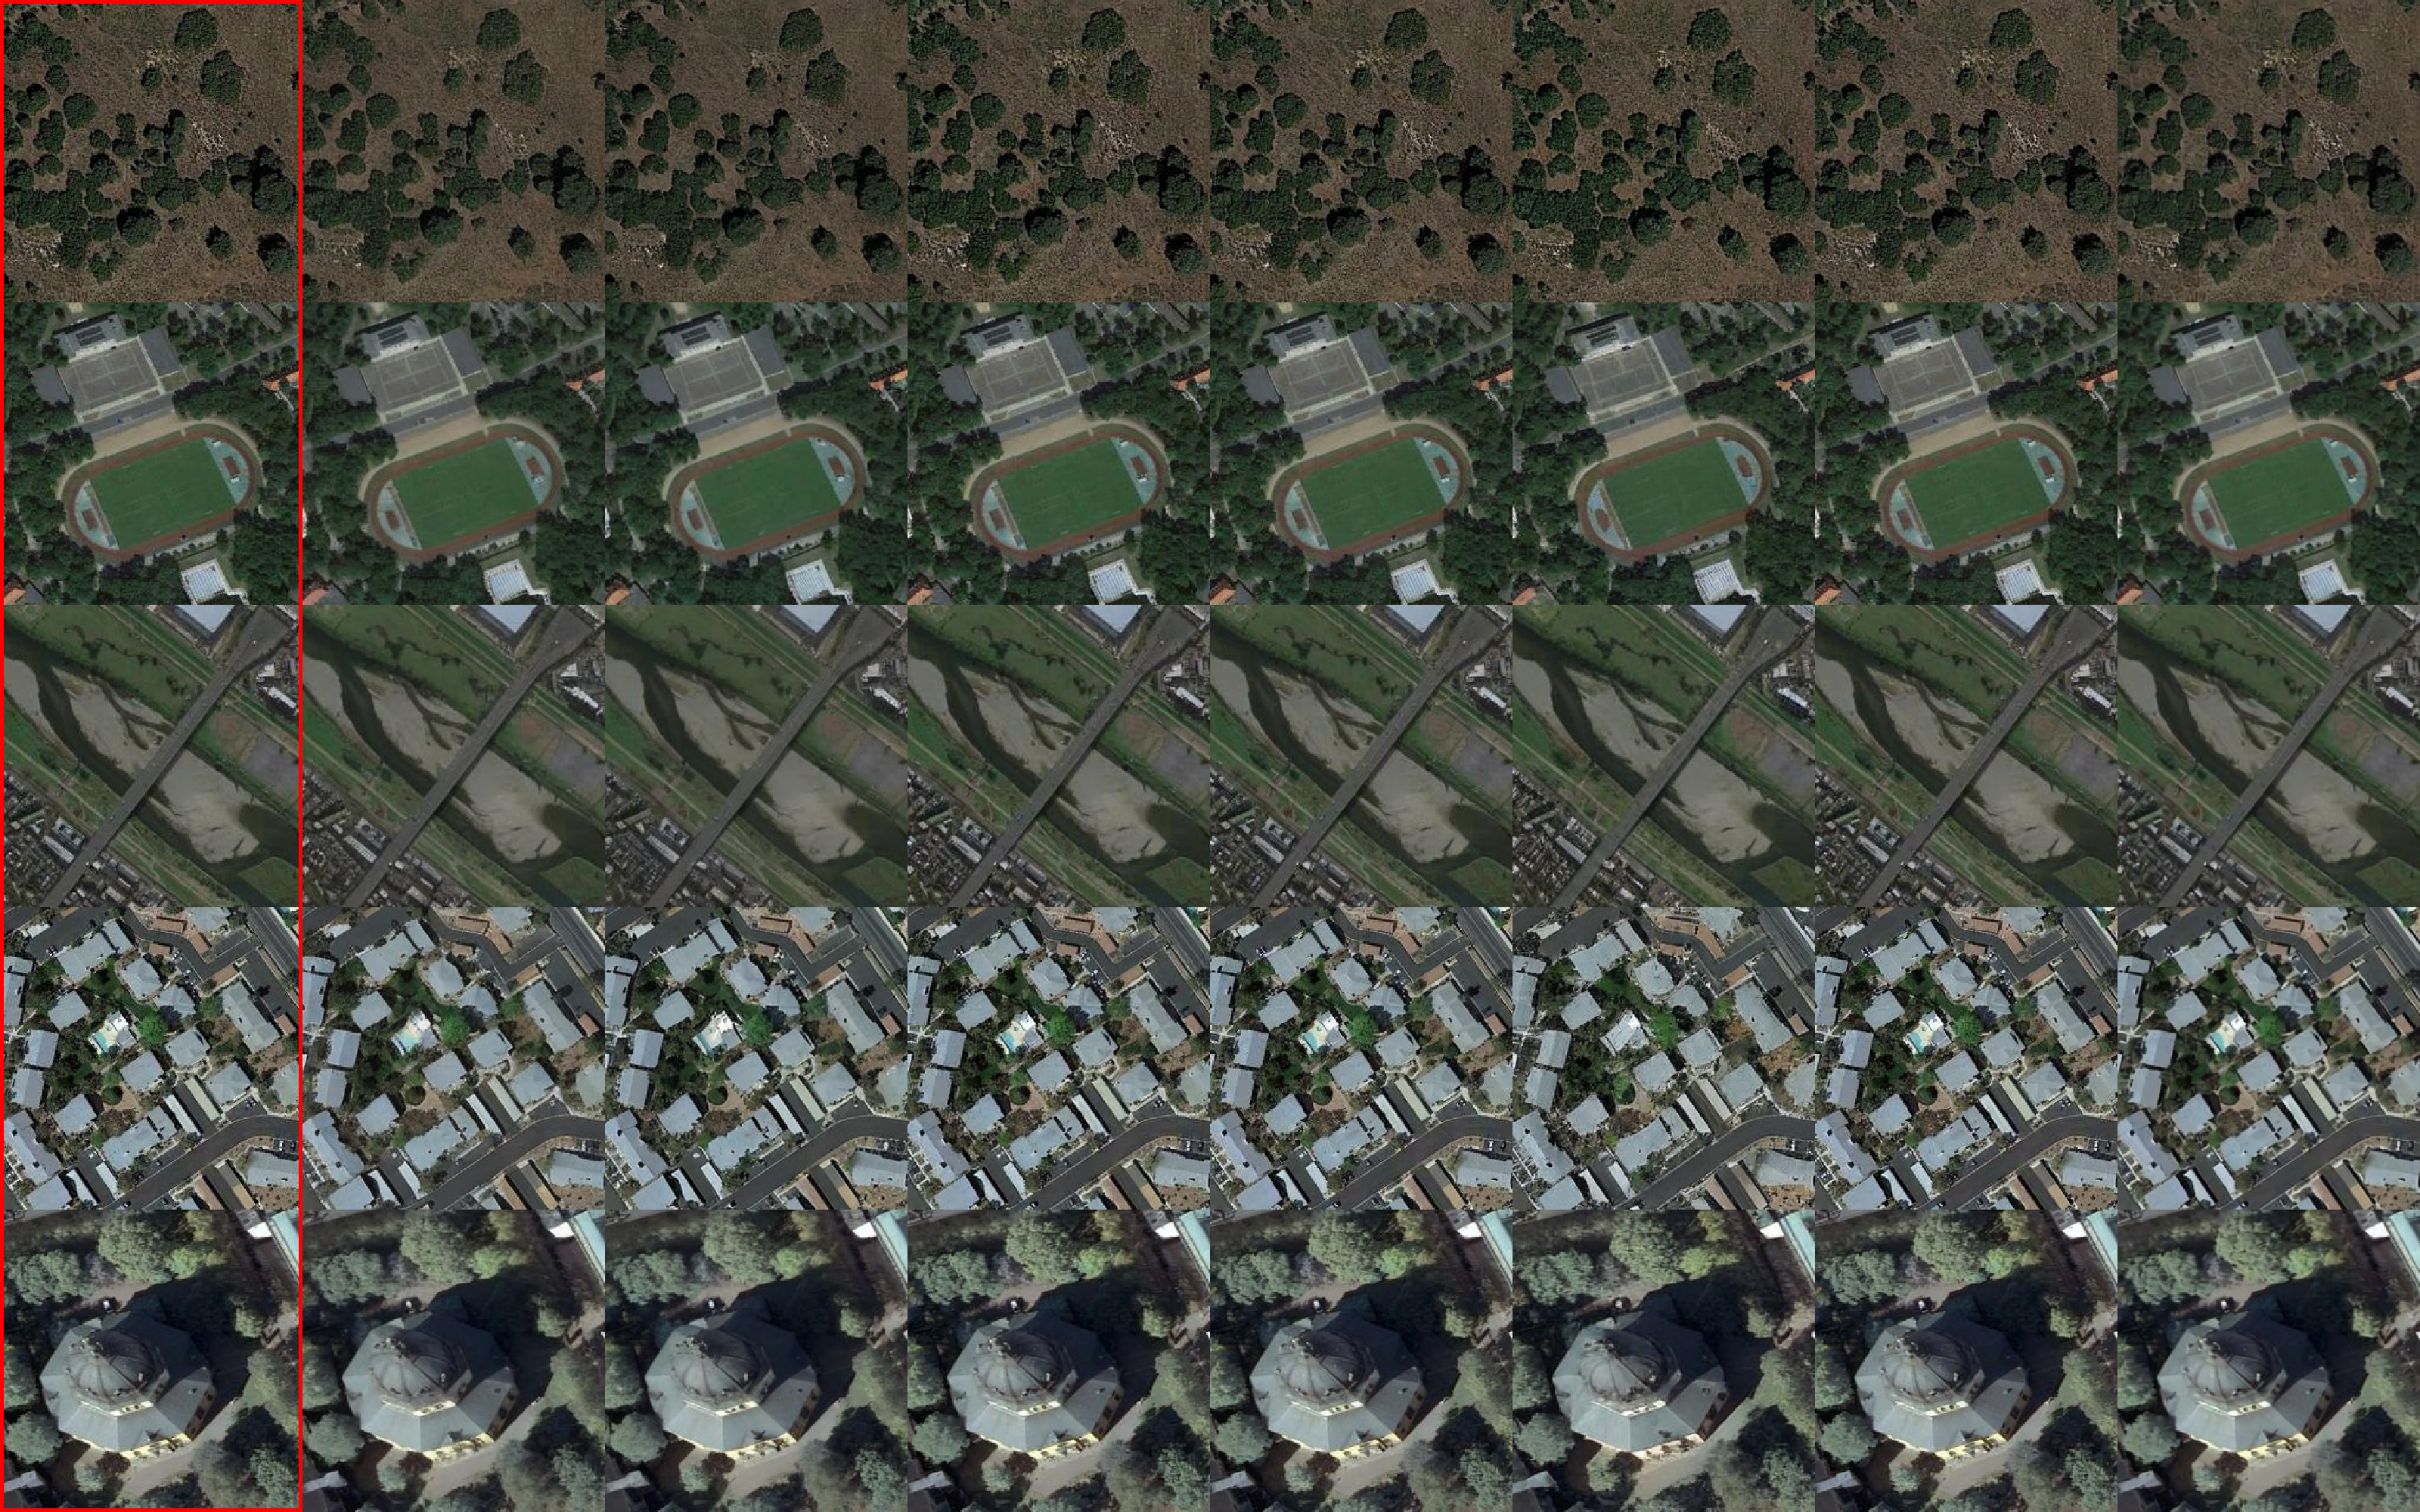
\includegraphics[width=1.0\textwidth]{figures/RESULT5samples.pdf}
    \caption{Qualitative reconstructions from 5 random RESISC45 samples. Each column shows (left to right): Original, SD21-VAE, SDXL-VAE, SD35-VAE, FLUX1-VAE, SANA-VAE, FLUX2-VAE, and Qwen-VAE. No significant visual difference appears.}
    \label{fig:main_comparison}
\end{figure}



\section{Insights}

Based on our extensive experiments, we highlight several key insights regarding the application of natural image VAEs to the remote sensing domain:

\begin{mybox}{Key Insights}
\begin{itemize}
    \item \textbf{Generalization of Natural Priors:} Standard VAEs pre-trained on ImageNet/LAION exhibit surprising robustness to RS data, suggesting that low-level visual features (edges, textures) are highly transferable across domains.
    \item \textbf{Model Architecture Matters:} Flow-matching based decoders (e.g., FLUX) provide significantly higher reconstruction fidelity for high-resolution satellite imagery compared to earlier KL-regularized architectures.
    \item \textbf{Zero-Shot Utility:} These models can serve as effective "cheap" pre-processors for denoising and initial data compression in RS pipelines without the need for expensive domain-specific re-training.
\end{itemize}
\end{mybox}

\section{Conclusion}

In this work, we explored the robustness of natural image priors in VAEs for remote sensing. Our findings indicate that these models, when used zero-shot, can provide significant utility in data compression and pre-processing tasks across various sensing categories. Future work could further explore the integration of domain-specific priors to enhance these capabilities.


\bibliography{iclr2026_conference}
\bibliographystyle{iclr2026_conference}

% \newpage
% \appendix
% \section{Appendix}
% If you choose to include an appendix, please submit it as a separate PDF file.

\end{document}
